% SemGuard (Wang 2025) workflow figure.
% Trained 1.3B classifier scores partial program after each line;
% rollback if score < 0.5. The evaluator is the only verifier --
% no compiler in the loop.
\documentclass[border=2pt]{standalone}
\usepackage{tikz}
\usepackage{xcolor}
\usetikzlibrary{shapes.geometric, arrows.meta, positioning, fit, backgrounds, calc}

\begin{document}
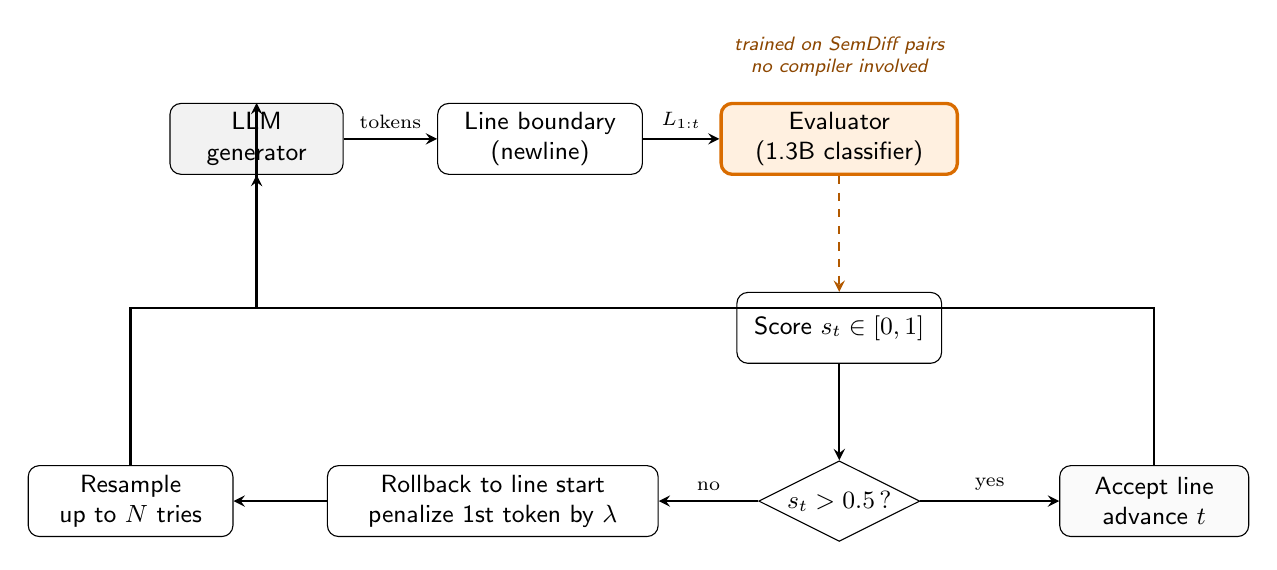
\begin{tikzpicture}[
    >=stealth,
    font=\sffamily\small,
    box/.style       ={draw, rounded corners, align=center, minimum height=9mm,
                       minimum width=26mm, inner sep=3pt, fill=white},
    llmbox/.style    ={box, fill=black!5, minimum width=22mm},
    learnbox/.style  ={box, draw=orange!85!black, very thick, fill=orange!12,
                       minimum width=30mm},
    decision/.style  ={diamond, draw, aspect=2.0, inner sep=1pt, align=center,
                       fill=white, minimum height=9mm},
    flow/.style      ={->, thick},
    softflow/.style  ={->, thick, orange!70!black, dashed},
    note/.style      ={font=\sffamily\scriptsize\itshape, text=orange!55!black}
]

% Top row: LLM -> line boundary -> evaluator
\node[llmbox]   (llm) at (0,0)   {LLM\\generator};
\node[box]      (nl)  at (3.6,0) {Line boundary\\(newline)};
\node[learnbox] (ev)  at (7.4,0) {Evaluator\\(1.3B classifier)};

\node[note, above=2mm of ev, text width=34mm, align=center]
    {trained on SemDiff pairs\\no compiler involved};

% Score + gate below evaluator
\node[box] (score) at (7.4,-2.4) {Score $s_t \in [0,1]$};
\node[decision] (gate) at (7.4,-4.6) {$s_t > 0.5\,?$};

% Accept branch (bottom-right)
\node[box, fill=black!2, minimum width=24mm] (ok) at (11.4,-4.6)
    {Accept line\\advance $t$};

% Penalty + Resample (bottom-left)
\node[box, minimum width=42mm] (pen) at (3.0,-4.6)
    {Rollback to line start\\penalize 1st token by $\lambda$};
\node[box] (rs) at (-1.6,-4.6) {Resample\\up to $N$ tries};

% --- Arrows ---
\draw[flow] (llm.east) -- (nl.west) node[midway, above, font=\scriptsize] {tokens};
\draw[flow] (nl.east) -- (ev.west)  node[midway, above, font=\scriptsize] {$L_{1:t}$};
\draw[softflow] (ev.south) -- (score.north);
\draw[flow] (score.south) -- (gate.north);

% Gate -> Accept
\draw[flow] (gate.east) -- (ok.west) node[midway, above, font=\scriptsize] {yes};
% Gate -> Rollback
\draw[flow] (gate.west) -- (pen.east) node[midway, above, font=\scriptsize] {no};
% Rollback -> Resample
\draw[flow] (pen.west) -- (rs.east);

% Accept -> LLM (back up along the right)
\draw[flow] (ok.north) -- ++(0,2.0) -| (llm.north)
    node[pos=0.08, right, font=\scriptsize] {};
% Resample -> LLM
\draw[flow] (rs.north) -- ++(0,2.0) -| (llm.south);

\end{tikzpicture}
\end{document}
